      \subsection{Návrh replikačního řešení}
      \label{kNavrh}

Po provedení rešeršní části a zohlednění všech podmínek, požadavků a možností katedry, byl sestaven návrh pro kompletní databázové řešení založené na procesu replikaci. Z databázových serverů, diskutovaných v kapitole \odkazKapitola{kPouziteProstredky}, byl vybrán server PostgreSQL hned z několika důvodů. Jedná se o plnohodnotný databázový systém dostupný zdarma se všemi nástroji, je široce používaný v oblasti geoinformačních technologií, je multiplatfomní a od verze ArcGIS 9.3 plně podporováný produkty ArcGIS. 

Byl navržen replikační cluster s nejméně třemi servery z důvodů, které již byly diskutovány v kapitole \odkazKapitola{kReplikace}. Celý cluster poběží na stejné platformě a proto bude možno použít streaming replikaci, která jakožto nativní řešení PostgreSQL, nabízí větší stabilitu a bezpečnost, díky přenosu transakčních logů, než jiná diskutovaná řešení. Byla zvolena jednosměrná master-slave replikace, cluster tedy bude obsahovat jeden master a dva (popř. více) slave serverů. Aby nedošlo ke ztrátě dat v případě, že by master server spadl dřív, než se data zkopírují na slave server, pro první slave (slave1) byla zvolena varianta synchronní replikace. Je vhodné, aby servery běžely v~lokální síti, protože se tím snižuje pravděpodobnost, že by došlo  k~výpadku spojení mezi master a slave1 server a nebylo by tak možno na master zapisovat. 

Druhý server (slave2) bude replikovat asynchronně a zároveň, aby nedocházelo k~přetížení master serveru, bude replikace probíhat ze slave1 na slave2, tedy kaskádově. Ze slave2 lze dále tvořit pravidelnou, například denní nebo týdenní, zálohu pomocí ulitily pg\_dump, která je více popsána v kapitole \odkazKapitola{kPriprava}. Záloha přes pg\_dump tak nebude zatěžovat master server a sama o sobě bude probíhat rychleji, než by tomu bylo na master serveru, který je již tak velmi vytížen dalšími procesy.

Uživatelé, kteří budou mít právo do databáze číst i zapisovat, se budou připojovat skrze pgpool, jehož výhody a možnosti byly popsány v kapitole \odkazKapitola{kpgpool}. Uživatelům to usnadní práci, protože si nebudou muset hlídat, ke kterému ze serverů se připojit na základě jejich aktuálního dotazu. pgpool se bude tvářit jako jakákoli jiná databáze, ke které se klienti přihlásí bez ohledu na typ jejich dotazu a on sám pak rozhodne, ke kterému ze serverů klienta přihlásí. Tím bude mít zároveň možnost rozložit zátěž na dostupné uzly v clusteru dle počtu konkrétních dotazů. Pro ještě větší efektivitu provozu databáze bude pgpool uchovávat databázová spojení a při novém dotazu využije stávajícího spojení, místo aby vytvářel spojení nové. Tímto se zajistí plynulost a zvýší rychlost provozu databáze.

      \begin{figure}[H]
        \label{oNavrhKatedra}
        \centering
        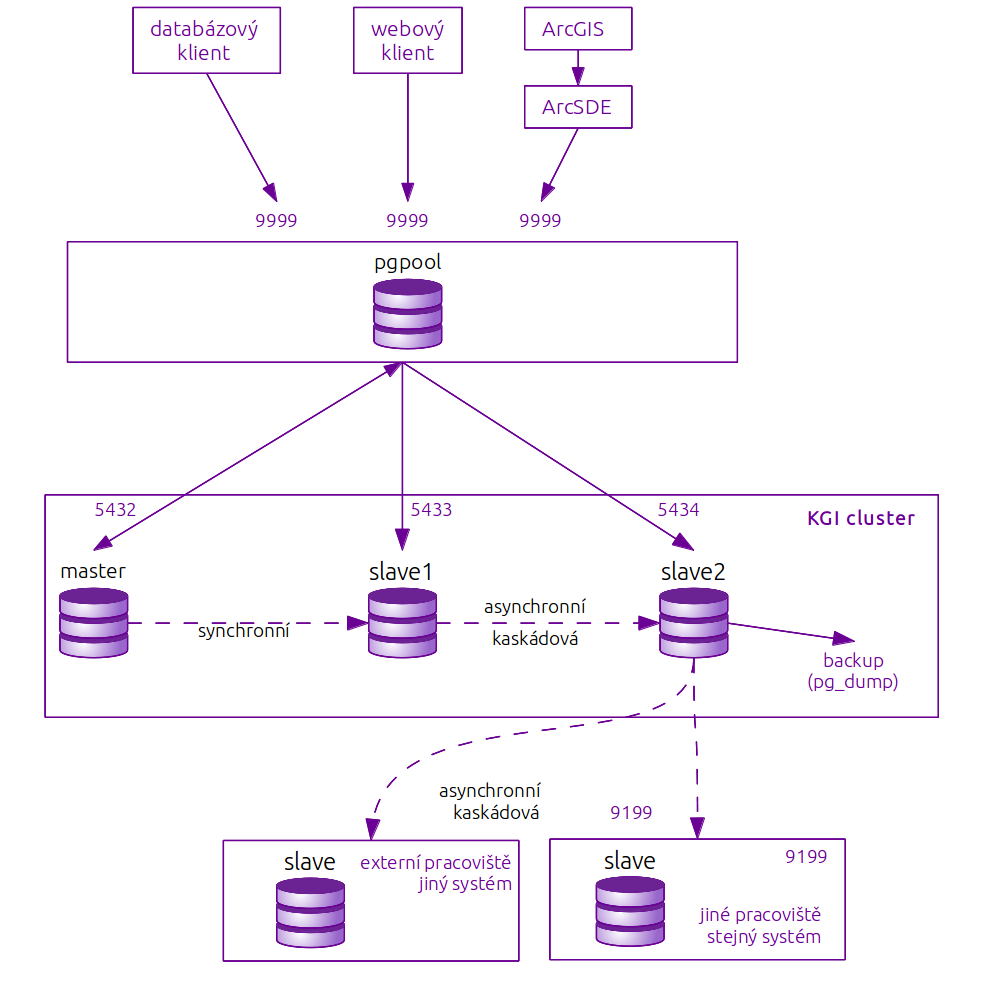
\includegraphics[scale=1]{../../../grafy/obr/schema_navrhKatedra2.png}
        \caption {Návrh replikačního řešení}
      \end{figure}

Vzhledem k tomu, že se klienti k databázi budou přistupovat skrze pgpool, není potřeba aby jednotlivé uzly v clusteru měly veřejnou IP adresu. Plně dostačuje, že servery poběží na lokální síti a pouze pgpool bude na serveru s veřejnou IP, čímž se zajistí, že data budou přístupná i skrze internet. 

Návrh počítá také s externími pracovišti, která budou často přistupovat do databáze s právem čtení, a budou mít zájem o zrychlení přístupu k datům tím, že se slave server přesune na jejich pracoviště, tedy na hardware, který bude připojen do jejich lokální sítě. Typ replikace se zvolí podle jejich operačního systému a jeho architektury. Pokud se bude jednat o shodný systém, jaký bude použit ve výše popsaném clusteru, pak bude možno použít asynchronní streaming replikaci, naopak pokud se bude bude jednat o systém jiný, bude použita Slony-I replikace. 

